\PassOptionsToPackage{unicode=true}{hyperref} % options for packages loaded elsewhere
\PassOptionsToPackage{hyphens}{url}
%
\documentclass[ignorenonframetext,]{beamer}
\usepackage{pgfpages}
\setbeamertemplate{caption}[numbered]
\setbeamertemplate{caption label separator}{: }
\setbeamercolor{caption name}{fg=normal text.fg}
\beamertemplatenavigationsymbolsempty
% Prevent slide breaks in the middle of a paragraph:
\widowpenalties 1 10000
\raggedbottom
\setbeamertemplate{part page}{
\centering
\begin{beamercolorbox}[sep=16pt,center]{part title}
  \usebeamerfont{part title}\insertpart\par
\end{beamercolorbox}
}
\setbeamertemplate{section page}{
\centering
\begin{beamercolorbox}[sep=12pt,center]{part title}
  \usebeamerfont{section title}\insertsection\par
\end{beamercolorbox}
}
\setbeamertemplate{subsection page}{
\centering
\begin{beamercolorbox}[sep=8pt,center]{part title}
  \usebeamerfont{subsection title}\insertsubsection\par
\end{beamercolorbox}
}
\AtBeginPart{
  \frame{\partpage}
}
\AtBeginSection{
  \ifbibliography
  \else
    \frame{\sectionpage}
  \fi
}
\AtBeginSubsection{
  \frame{\subsectionpage}
}
\usepackage{lmodern}
\usepackage{amssymb,amsmath}
\usepackage{ifxetex,ifluatex}
\usepackage{fixltx2e} % provides \textsubscript
\ifnum 0\ifxetex 1\fi\ifluatex 1\fi=0 % if pdftex
  \usepackage[T1]{fontenc}
  \usepackage[utf8]{inputenc}
  \usepackage{textcomp} % provides euro and other symbols
\else % if luatex or xelatex
  \usepackage{unicode-math}
  \defaultfontfeatures{Ligatures=TeX,Scale=MatchLowercase}
\fi
\usecolortheme{seahorse}
% use upquote if available, for straight quotes in verbatim environments
\IfFileExists{upquote.sty}{\usepackage{upquote}}{}
% use microtype if available
\IfFileExists{microtype.sty}{%
\usepackage[]{microtype}
\UseMicrotypeSet[protrusion]{basicmath} % disable protrusion for tt fonts
}{}
\IfFileExists{parskip.sty}{%
\usepackage{parskip}
}{% else
\setlength{\parindent}{0pt}
\setlength{\parskip}{6pt plus 2pt minus 1pt}
}
\usepackage{hyperref}
\hypersetup{
            pdftitle={Quantitative Drama Analytics},
            pdfauthor={Nils Reiter},
            pdfborder={0 0 0},
            breaklinks=true}
\urlstyle{same}  % don't use monospace font for urls
\newif\ifbibliography
\usepackage{color}
\usepackage{fancyvrb}
\newcommand{\VerbBar}{|}
\newcommand{\VERB}{\Verb[commandchars=\\\{\}]}
\DefineVerbatimEnvironment{Highlighting}{Verbatim}{commandchars=\\\{\}}
% Add ',fontsize=\small' for more characters per line
\usepackage{framed}
\definecolor{shadecolor}{RGB}{248,248,248}
\newenvironment{Shaded}{\begin{snugshade}}{\end{snugshade}}
\newcommand{\AlertTok}[1]{\textcolor[rgb]{0.94,0.16,0.16}{#1}}
\newcommand{\AnnotationTok}[1]{\textcolor[rgb]{0.56,0.35,0.01}{\textbf{\textit{#1}}}}
\newcommand{\AttributeTok}[1]{\textcolor[rgb]{0.77,0.63,0.00}{#1}}
\newcommand{\BaseNTok}[1]{\textcolor[rgb]{0.00,0.00,0.81}{#1}}
\newcommand{\BuiltInTok}[1]{#1}
\newcommand{\CharTok}[1]{\textcolor[rgb]{0.31,0.60,0.02}{#1}}
\newcommand{\CommentTok}[1]{\textcolor[rgb]{0.56,0.35,0.01}{\textit{#1}}}
\newcommand{\CommentVarTok}[1]{\textcolor[rgb]{0.56,0.35,0.01}{\textbf{\textit{#1}}}}
\newcommand{\ConstantTok}[1]{\textcolor[rgb]{0.00,0.00,0.00}{#1}}
\newcommand{\ControlFlowTok}[1]{\textcolor[rgb]{0.13,0.29,0.53}{\textbf{#1}}}
\newcommand{\DataTypeTok}[1]{\textcolor[rgb]{0.13,0.29,0.53}{#1}}
\newcommand{\DecValTok}[1]{\textcolor[rgb]{0.00,0.00,0.81}{#1}}
\newcommand{\DocumentationTok}[1]{\textcolor[rgb]{0.56,0.35,0.01}{\textbf{\textit{#1}}}}
\newcommand{\ErrorTok}[1]{\textcolor[rgb]{0.64,0.00,0.00}{\textbf{#1}}}
\newcommand{\ExtensionTok}[1]{#1}
\newcommand{\FloatTok}[1]{\textcolor[rgb]{0.00,0.00,0.81}{#1}}
\newcommand{\FunctionTok}[1]{\textcolor[rgb]{0.00,0.00,0.00}{#1}}
\newcommand{\ImportTok}[1]{#1}
\newcommand{\InformationTok}[1]{\textcolor[rgb]{0.56,0.35,0.01}{\textbf{\textit{#1}}}}
\newcommand{\KeywordTok}[1]{\textcolor[rgb]{0.13,0.29,0.53}{\textbf{#1}}}
\newcommand{\NormalTok}[1]{#1}
\newcommand{\OperatorTok}[1]{\textcolor[rgb]{0.81,0.36,0.00}{\textbf{#1}}}
\newcommand{\OtherTok}[1]{\textcolor[rgb]{0.56,0.35,0.01}{#1}}
\newcommand{\PreprocessorTok}[1]{\textcolor[rgb]{0.56,0.35,0.01}{\textit{#1}}}
\newcommand{\RegionMarkerTok}[1]{#1}
\newcommand{\SpecialCharTok}[1]{\textcolor[rgb]{0.00,0.00,0.00}{#1}}
\newcommand{\SpecialStringTok}[1]{\textcolor[rgb]{0.31,0.60,0.02}{#1}}
\newcommand{\StringTok}[1]{\textcolor[rgb]{0.31,0.60,0.02}{#1}}
\newcommand{\VariableTok}[1]{\textcolor[rgb]{0.00,0.00,0.00}{#1}}
\newcommand{\VerbatimStringTok}[1]{\textcolor[rgb]{0.31,0.60,0.02}{#1}}
\newcommand{\WarningTok}[1]{\textcolor[rgb]{0.56,0.35,0.01}{\textbf{\textit{#1}}}}
\usepackage{longtable,booktabs}
\usepackage{caption}
% These lines are needed to make table captions work with longtable:
\makeatletter
\def\fnum@table{\tablename~\thetable}
\makeatother
\usepackage{graphicx,grffile}
\makeatletter
\def\maxwidth{\ifdim\Gin@nat@width>\linewidth\linewidth\else\Gin@nat@width\fi}
\def\maxheight{\ifdim\Gin@nat@height>\textheight\textheight\else\Gin@nat@height\fi}
\makeatother
% Scale images if necessary, so that they will not overflow the page
% margins by default, and it is still possible to overwrite the defaults
% using explicit options in \includegraphics[width, height, ...]{}
\setkeys{Gin}{width=\maxwidth,height=\maxheight,keepaspectratio}
\setlength{\emergencystretch}{3em}  % prevent overfull lines
\providecommand{\tightlist}{%
  \setlength{\itemsep}{0pt}\setlength{\parskip}{0pt}}
\setcounter{secnumdepth}{0}

% set default figure placement to htbp
\makeatletter
\def\fps@figure{htbp}
\makeatother

\usepackage{booktabs}

\setbeamertemplate{itemize items}[circle]

\title{Quantitative Drama Analytics}
\providecommand{\subtitle}[1]{}
\subtitle{Part 2: lab session}
\author{Nils Reiter}
\date{July 15, 2019}

\begin{document}
\frame{\titlepage}

\hypertarget{what-you-really-need-to-know-about-r}{%
\section{What you really need to know about
R}\label{what-you-really-need-to-know-about-r}}

\begin{frame}{R Basics}
\protect\hypertarget{r-basics}{}

\begin{itemize}
\tightlist
\item
  R is a programming language

  \begin{itemize}
  \tightlist
  \item
    Mostly used for statistical data analysis (``data science'')
  \item
    First version: 1993
  \item
    Current stable release: 3.6
  \item
    \href{https://www.r-project.org/}{Website}
  \end{itemize}
\item
  Three important concepts we need to talk about

  \begin{itemize}
  \tightlist
  \item
    Objects/Types
  \item
    Variables
  \item
    Functions
  \end{itemize}
\end{itemize}

\end{frame}

\begin{frame}[fragile]{R Basics}
\protect\hypertarget{r-basics-1}{}

\framesubtitle{Objects and Types}

\begin{itemize}
\tightlist
\item
  Objects live in the computer memory (or on disk)
\item
  Objects represent the things we want to analyse (e.g., dramatic texts,
  words, or numbers)
\item
  An object has one or more types
\item
  The type of an object determines what we can do with it

  \begin{itemize}
  \tightlist
  \item
    E.g., a knife allows other operations than a fork \pause
  \end{itemize}
\item
  Types: Numbers, strings, lists, tables, \ldots{}

  \begin{itemize}
  \tightlist
  \item
    Numbers allow arithmetic operations

    \begin{itemize}
    \tightlist
    \item
      E.g., summation: \texttt{sum(3,5)} (evaluates to \texttt{8},
      equivalent to \texttt{3+5})
    \end{itemize}
  \item
    Strings allow character-based operations

    \begin{itemize}
    \tightlist
    \item
      E.g., conversion to lower case: \texttt{tolower("ABC")} (evaluates
      to \texttt{"abc"}) \pause
    \end{itemize}
  \end{itemize}
\item
  ``evalutes to'': result of the operation
\end{itemize}

\end{frame}

\begin{frame}[fragile]{R Basics}
\protect\hypertarget{r-basics-2}{}

\framesubtitle{Objects and Types}

\small

\begin{longtable}[]{@{}lll@{}}
\toprule
Type & Example & Description\tabularnewline
\midrule
\endhead
Numeric & \texttt{5} & A numeric value\tabularnewline
Character & \texttt{"Heidelberg"} & A sequence of
characters\tabularnewline
& & (note the double quotes!)\tabularnewline
Logical & \texttt{TRUE}/\texttt{FALSE} & A truth value\tabularnewline
Vector & \texttt{c(5,4,1)} & Sequence of objects \emph{of the same
type}\tabularnewline
List & \texttt{list(5,"Hd",TRUE)} & Sequence of objects\tabularnewline
Matrix & & Table of objects \emph{of the same type}\tabularnewline
Data frame & & Table of objects\tabularnewline
\bottomrule
\end{longtable}

\end{frame}

\begin{frame}[fragile]{R Basics}
\protect\hypertarget{r-basics-3}{}

\framesubtitle{Objects and Types}

In R, everything is a vector!

\begin{itemize}
\tightlist
\item
  Entering \texttt{5} creates a numeric vector of length 1
\item
  Entering \texttt{"Bla"} creates a character vector of length 1
\end{itemize}

(In this way, R is different from other programming languages)

\begin{Shaded}
\begin{Highlighting}[]
\DecValTok{5}
\CommentTok{# Creates a vector consisting of the numbers 1 to 50}
\DecValTok{1}\OperatorTok{:}\DecValTok{50}
\end{Highlighting}
\end{Shaded}

\end{frame}

\begin{frame}[fragile]{R Basics}
\protect\hypertarget{r-basics-4}{}

\framesubtitle{Variables}

\begin{itemize}
\tightlist
\item
  We usually do not interact with the objects directly

  \begin{itemize}
  \tightlist
  \item
    Because they are not known in advance (but loaded from files)
  \end{itemize}
\item
  Variables

  \begin{itemize}
  \tightlist
  \item
    A way to \emph{name} objects
  \item
    Used as a placeholder for objects
  \item
    The actual operation takes place on the objects (R takes care of
    this)
  \end{itemize}
\item
  Creating a variable \texttt{a}: \texttt{a\ \textless{}-\ 3} (think of
  this as an arrow)
\end{itemize}

\begin{Shaded}
\begin{Highlighting}[]
\OperatorTok{>}\StringTok{ }\NormalTok{a <-}\StringTok{ }\DecValTok{3}
\OperatorTok{>}\StringTok{ }\NormalTok{b <-}\StringTok{ }\DecValTok{5}
\OperatorTok{>}\StringTok{ }\NormalTok{a }\OperatorTok{+}\StringTok{ }\NormalTok{b}
\NormalTok{[}\DecValTok{1}\NormalTok{] }\DecValTok{8}
\OperatorTok{>}
\end{Highlighting}
\end{Shaded}

\end{frame}

\begin{frame}[fragile]{R Basics}
\protect\hypertarget{r-basics-5}{}

\framesubtitle{Functions}

\begin{itemize}
\tightlist
\item
  ``Mini programs'': A collection of instructions that you can use as a
  single instruction
\item
  Input: Functions take \emph{arguments} as input
\item
  Output: Functions return an object (that stores the result of the
  instructions) \pause
\item
  Functions have a name (typically lower case) and can be reognized by
  the round parentheses\\
  \texttt{function(argument1,\ argument2,\ argument3,\ ...)}
\item
  The return value of a function can be stored in a variable\\
  \texttt{variable\ \textless{}-\ function(arg1,\ arg2,\ ...)} \pause
\item
  Some functions not only return a value, but also do something (e.g.,
  display a plot)
\end{itemize}

\end{frame}

\begin{frame}[fragile]{R Basics}
\protect\hypertarget{r-basics-6}{}

\framesubtitle{Functions}

\begin{Shaded}
\begin{Highlighting}[]
\KeywordTok{sum}\NormalTok{(}\DecValTok{5}\NormalTok{,}\DecValTok{1}\NormalTok{)         }\CommentTok{# 5 + 1 is only an abbreviation}
\NormalTok{s <-}\StringTok{ }\KeywordTok{sum}\NormalTok{(}\DecValTok{5}\NormalTok{,}\DecValTok{1}\NormalTok{)    }\CommentTok{# stores the result in a }
                 \CommentTok{# variable, no output}
\NormalTok{s                }\CommentTok{# prints the value of the variable}
\NormalTok{s <-}\StringTok{ }\DecValTok{7}           \CommentTok{# overwrites the previous value of }
                 \CommentTok{# the variable}
\NormalTok{s <-}\StringTok{ }\KeywordTok{sum}\NormalTok{(s,}\DecValTok{3}\NormalTok{)    }\CommentTok{# overwrites the value of the }
                 \CommentTok{# variable}
\end{Highlighting}
\end{Shaded}

What is the value of \texttt{s} now?

\end{frame}

\hypertarget{rstudio}{%
\subsection{RStudio}\label{rstudio}}

\begin{frame}{RStudio}
\protect\hypertarget{rstudio-1}{}

\begin{itemize}
\tightlist
\item
  An integrated development environment (IDE) for R
\item
  Capable workbench for data analysis
\end{itemize}

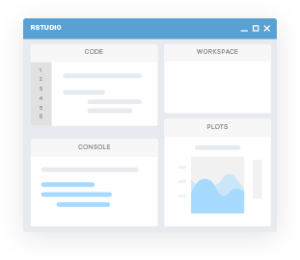
\includegraphics{rstudio-300x260.png}
\{height=0.3\textbackslash{}textheight\}

\end{frame}

\begin{frame}{RStudio}
\protect\hypertarget{rstudio-2}{}

\framesubtitle{Four Panes}

\begin{itemize}
\tightlist
\item
  Console: Where you enter R code and get the result immediately
\item
  Environment: Shows the objects currently in memory
\item
  Plots: Shows plots
\item
  Editor/Code: Allows editing R code and inspecting tables
\end{itemize}

We will focus on the console and plot area

\end{frame}

\hypertarget{dramaanalysis}{%
\section{DramaAnalysis}\label{dramaanalysis}}

\begin{frame}{Outline}
\protect\hypertarget{outline}{}

\begin{itemize}
\tightlist
\item
  Introduction/Installation and Overview
\item
  Three areas for you to play with

  \begin{enumerate}
  \tightlist
  \item
    General character statistics
  \item
    Word fields
  \item
    Copresence and network analysis
  \end{enumerate}
\end{itemize}

\end{frame}

\begin{frame}{Introduction}
\protect\hypertarget{introduction}{}

\begin{itemize}
\tightlist
\item
  \url{https://quadrama.github.io/DramaAnalysis/tutorial/3/}
\end{itemize}

\end{frame}

\hypertarget{installation}{%
\subsection{Installation}\label{installation}}

\begin{frame}[fragile]{Installation}
\protect\hypertarget{installation-1}{}

\framesubtitle{Code}

\begin{Shaded}
\begin{Highlighting}[]
\KeywordTok{install.packages}\NormalTok{(}\StringTok{"DramaAnalysis"}\NormalTok{)}
\KeywordTok{library}\NormalTok{(DramaAnalysis)  }\CommentTok{# no quotes}

\KeywordTok{library}\NormalTok{(magrittr) }\CommentTok{# additional package}
\end{Highlighting}
\end{Shaded}

\end{frame}

\begin{frame}[fragile]{Installation}
\protect\hypertarget{installation-2}{}

\framesubtitle{Data}

\begin{itemize}
\tightlist
\item
  Dramatic texts are initially stored as TEI/XML files
\item
  Language processing (e.g., detection of parts of speech) takes place
  in a UIMA pipeline
\item
  The output of the pipeline are several CSV files for each play (meta
  data, character data, \dots)
\item
  CSV files are then analysed in R
\end{itemize}

\pause

Two corpora today:

\begin{Shaded}
\begin{Highlighting}[]
\KeywordTok{installData}\NormalTok{(}\StringTok{"qd"}\NormalTok{) }\CommentTok{# German literary canon}
\CommentTok{# or}
\KeywordTok{installData}\NormalTok{(}\StringTok{"shakedracor"}\NormalTok{) }\CommentTok{# English Shakespeare plays}
\end{Highlighting}
\end{Shaded}

\end{frame}

\begin{frame}[fragile]{Installation}
\protect\hypertarget{installation-3}{}

\framesubtitle{Data}

The function \texttt{installData()}

\begin{itemize}
\tightlist
\item
  Clones a git repository from \texttt{github.com/quadrama} into a local
  directory
\item
  Allows easy update of data files
\item
  German literary canon (\texttt{qd})

  \begin{itemize}
  \tightlist
  \item
    TextGrid, GerDraCor, QuaDramA
  \end{itemize}
\item
  English Shakespeare plays (\texttt{shakedracor})

  \begin{itemize}
  \tightlist
  \item
    Folger, DraCor, QuaDramA
  \end{itemize}
\end{itemize}

\end{frame}

\begin{frame}[fragile]{Loading a play}
\protect\hypertarget{loading-a-play}{}

\begin{itemize}
\tightlist
\item
  We first have to load plays into the environment
\item
  Each play has an associated id
\item
  Select one and create a variable to store the id (less typing in the
  future)
\end{itemize}

\pause

\begin{Shaded}
\begin{Highlighting}[]
\NormalTok{myId <-}\StringTok{ "shakedracor:romeo-and-juliet"}

\NormalTok{play <-}\StringTok{ }\KeywordTok{loadDrama}\NormalTok{(myId)}
\end{Highlighting}
\end{Shaded}

\end{frame}

\hypertarget{what-can-we-do}{%
\subsection{What can we do?}\label{what-can-we-do}}

\begin{frame}{Function overview}
\protect\hypertarget{function-overview}{}

\includegraphics{workflow.pdf}

\end{frame}

\hypertarget{global-character-statistics}{%
\subsection{1. Global character
statistics}\label{global-character-statistics}}

\begin{frame}[fragile]{Global character statistics}
\protect\hypertarget{global-character-statistics-1}{}

Two functions:

\begin{itemize}
\tightlist
\item
  \texttt{characterStatistics()}: Characters in focus
\item
  \texttt{utteranceStatistics()}: Utterances in focus
\end{itemize}

\end{frame}

\begin{frame}[fragile]{Function \texttt{characterStatistics}}
\protect\hypertarget{function-characterstatistics}{}

\begin{Shaded}
\begin{Highlighting}[]
\NormalTok{cs <-}\StringTok{ }\KeywordTok{characterStatistics}\NormalTok{(play)}
\end{Highlighting}
\end{Shaded}

Returns a table with

\begin{itemize}
\tightlist
\item
  \texttt{drama}: The play id
\item
  \texttt{character}: the character id
\item
  \texttt{tokens}: Number of tokens (for this character)
\item
  \texttt{types}: Number of different tokens (for this character)
\item
  \texttt{utterances}: Number of utterances (for this character)
\item
  \texttt{utteranceLengthMean}: Mean utterance length
\item
  \texttt{utteranceLengthSd}: Utterance length standard deviation
\item
  \texttt{firstBegin}: Starting position of the first utterance
\item
  \texttt{lastEnd}: End position of the last utterance
\end{itemize}

\end{frame}

\begin{frame}[fragile]{Function \texttt{characterStatistics}}
\protect\hypertarget{function-characterstatistics-1}{}

\framesubtitle{Plotting}

\begin{Shaded}
\begin{Highlighting}[]
\KeywordTok{characterStatistics}\NormalTok{(rksp}\FloatTok{.0}\NormalTok{) }\OperatorTok
\StringTok{  }\KeywordTok{characterNames}\NormalTok{(rksp}\FloatTok{.0}\NormalTok{) }\OperatorTok
\StringTok{  }\KeywordTok{barplot}\NormalTok{()}
\end{Highlighting}
\end{Shaded}

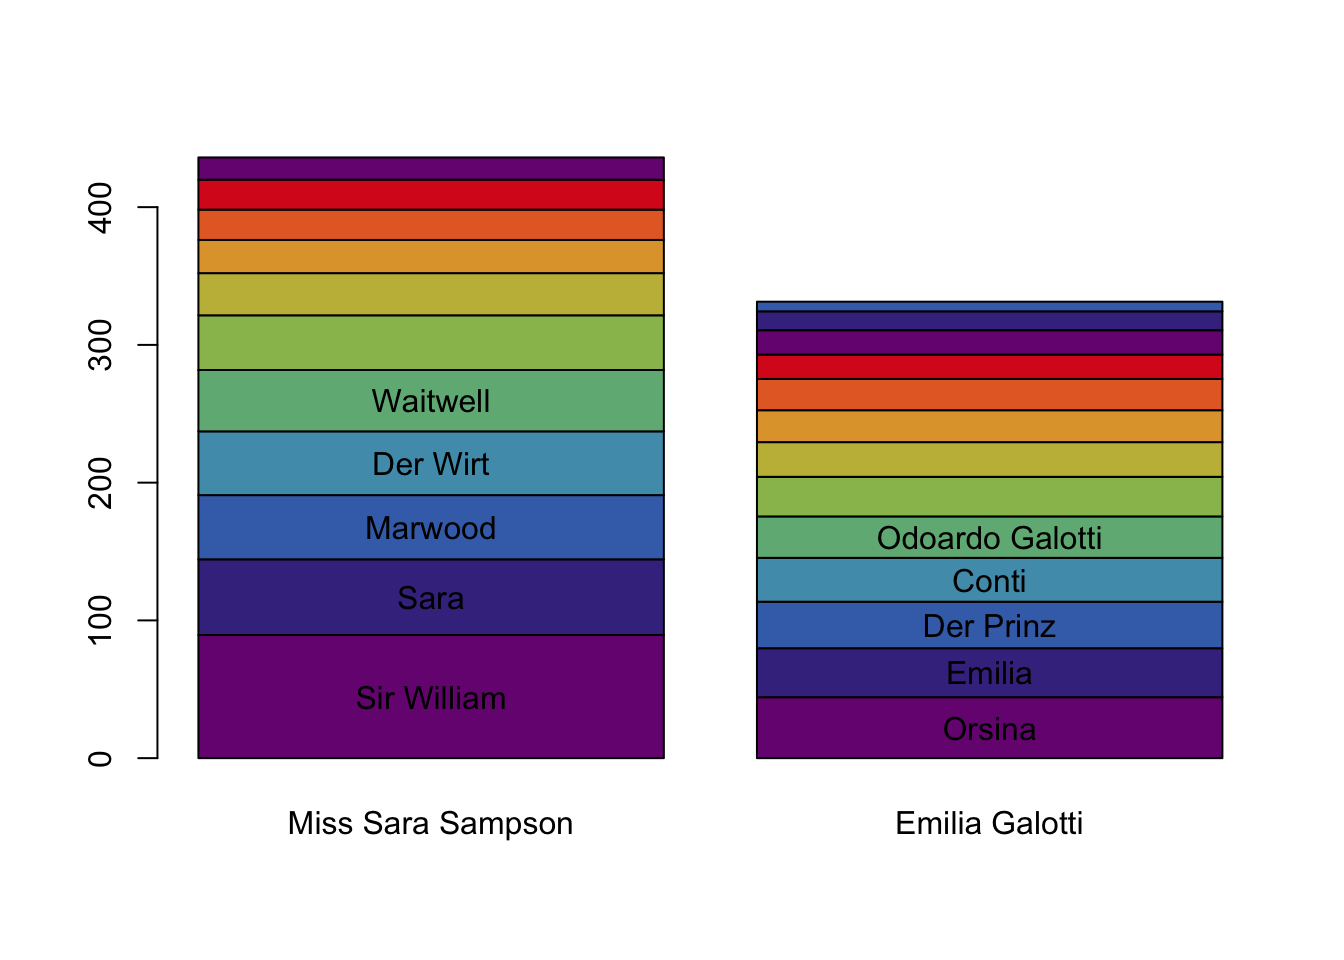
\includegraphics[height=0.6\textheight]{slides_files/figure-beamer/unnamed-chunk-7-1}

\end{frame}

\end{document}
